
\documentclass[11pt]{article}
\usepackage[margin=1in]{geometry}
\usepackage{hyperref}
\usepackage{graphicx}
\usepackage{amsmath}
\usepackage{enumitem}
\usepackage{listings}
\usepackage{xcolor}
\usepackage{draftwatermark}
\SetWatermarkText{DRAFT}
\SetWatermarkScale{3}
\SetWatermarkColor[gray]{0.85}

\definecolor{lightgray}{gray}{0.95}
\lstset{
  basicstyle=\ttfamily\small,
  backgroundcolor=\color{lightgray},
  breaklines=true,
  columns=fullflexible
}

\title{IPv6-Only HTCondor Integration with the Open Science Pool: \\
The Viper Cluster at GW/CAAREN}
\author{Research Technology Services, GWIT\\
The George Washington University}
\date{\today}

\begin{document}

\maketitle

\section{Introduction}

In 2025,  The George Washington University~\cite{gwu}, in partnership with the Capital Area Advanced Research and Education Network (CAAREN)~\cite{caaren},  
\href{https://ce-dashboard.ospool.osg-htc.org/overview.html?host=gwu-viper-ce1&r=week}{successfully} 
contributed a single-stack IPv6 HTCondor~\cite{htcondor} cluster, Viper, to the Open Science Pool (OSPool)~\cite{ospool}, a nationally distributed computing platform for data-intensive research. This demonstrates a path forward for institutions preparing for an IPv6-only future, reinforcing GW’s leadership in research cyberinfrastructure and open science.

There is some legitimate concern that integrating IPv6-only computational resources into the OSPool may have adverse effects on effective job-throughput. These concerns break down into two broad categories, 
\begin{enumerate}[itemsep=1pt]
\item Interoperability with OSPool and HTCondor 
\item Interoperability with researcher jobs which are far less predictable
\end{enumerate}

\section{System Overview}

Viper is a 12-node HTCondor cluster managed with Warewulf 4.6.1~\cite{warewulf} running Rocky Linux 9.5 and supported by a dedicated network-attached ZFS pool for backups and administrative workflows.  Each node in the cluster is a Dell PowerEdge R730 with the following hardware specifications:

\begin{center}
\small
\begin{tabular}{|l|l|}
\hline
\textbf{Component} & \textbf{Specification} \\
\hline
Cores & 2x14 Intel Xeon E5-2680 v4 @ 2.40GHz\\
RAM & 8x16 GB DIMM ECC 2400 MT/s \\
Scratch Storage & 1 TB SSD \\
\hline
\end{tabular}
\end{center}
There  are two master nodes serving as redundant central-managers in an active-passive relation, one
submit node, and nine execute points. Because Viper uses Warewulf's stateless provisioning, nodes can be quickly repurposed or recovered after failure.

Viper is configured to advertise 4.5 GB of RAM per core to the Open Science Pool, allowing it to efficiently integrate with workloads of varying shapes.  All Viper hosts have globally routable IPv6 addresses through CAAREN. 

\section{About CAAREN}

The Capital Area Advanced Research and Education Network (CAAREN) provides high-performance networking to support education, research, and innovation in the Washington, D.C. area. As a regional optical network and member of Internet2, CAAREN connects GW to other research institutions and to global science collaborations.
\newline

CAAREN has been a leader in routing security, being among the first US higher education institutions to implement Route Origin Authorization (ROAs).  CAAREN implemented the first know production deployment of TCP-AO for advanced BGP session security~\cite{TCPAO}.
\newline

Also available on CAAREN is an advanced content distribution test environment using Tree Distribution Networking (TreeDN)~\cite{TreeDN}.  Employing a combination of native multicast and overlay tunneling technology (via Automatic Multicast Tunneling - AMT), multicast content can be delivered to any endpoint.
\newline

CAAREN’s core network includes:
\begin{itemize}[leftmargin=*,itemsep=1pt]
 \item Juniper MX480 
\item DWDM with optical protection to connect to Intenet2
 \item Supplemental 10 Gbps access via secondary switches
\end{itemize}

Additional CAAREN services include:
\begin{itemize}[leftmargin=*,label=–,itemsep=1pt]
 \item Cloud Connect: Dedicated links via Internet2’s footprint to AWS, Azure, Google Cloud, and OCI, offering low-latency, secure access to cloud resources.
 \item The Things Network: A collaborative IoT sensor network initiative using LoRaWAN for low-power, long-range device communication.
\end{itemize}

These services position CAAREN as a leader for data-intensive science, advanced networking research, and the transition to secure, scalable IPv6-only architectures.

\section{Network Architecture}
\begin{itemize}[leftmargin=*,label=–,itemsep=1pt]
 \item \textbf{CAAREN Connectivity:} Global IPv6 /64 allocations routed through CAAREN. All Condor daemon communication (Collector, Negotiator, StartD, Schedd) operates exclusively over native IPv6.
 \item \textbf{Firewalls:} Host-based firewall rules allowing limited IPv6 originating from both GW and OSG and unrestricted outbound. No other firewalls or access control lists.
\end{itemize}

\begin{figure}[htbp]
  \centering
  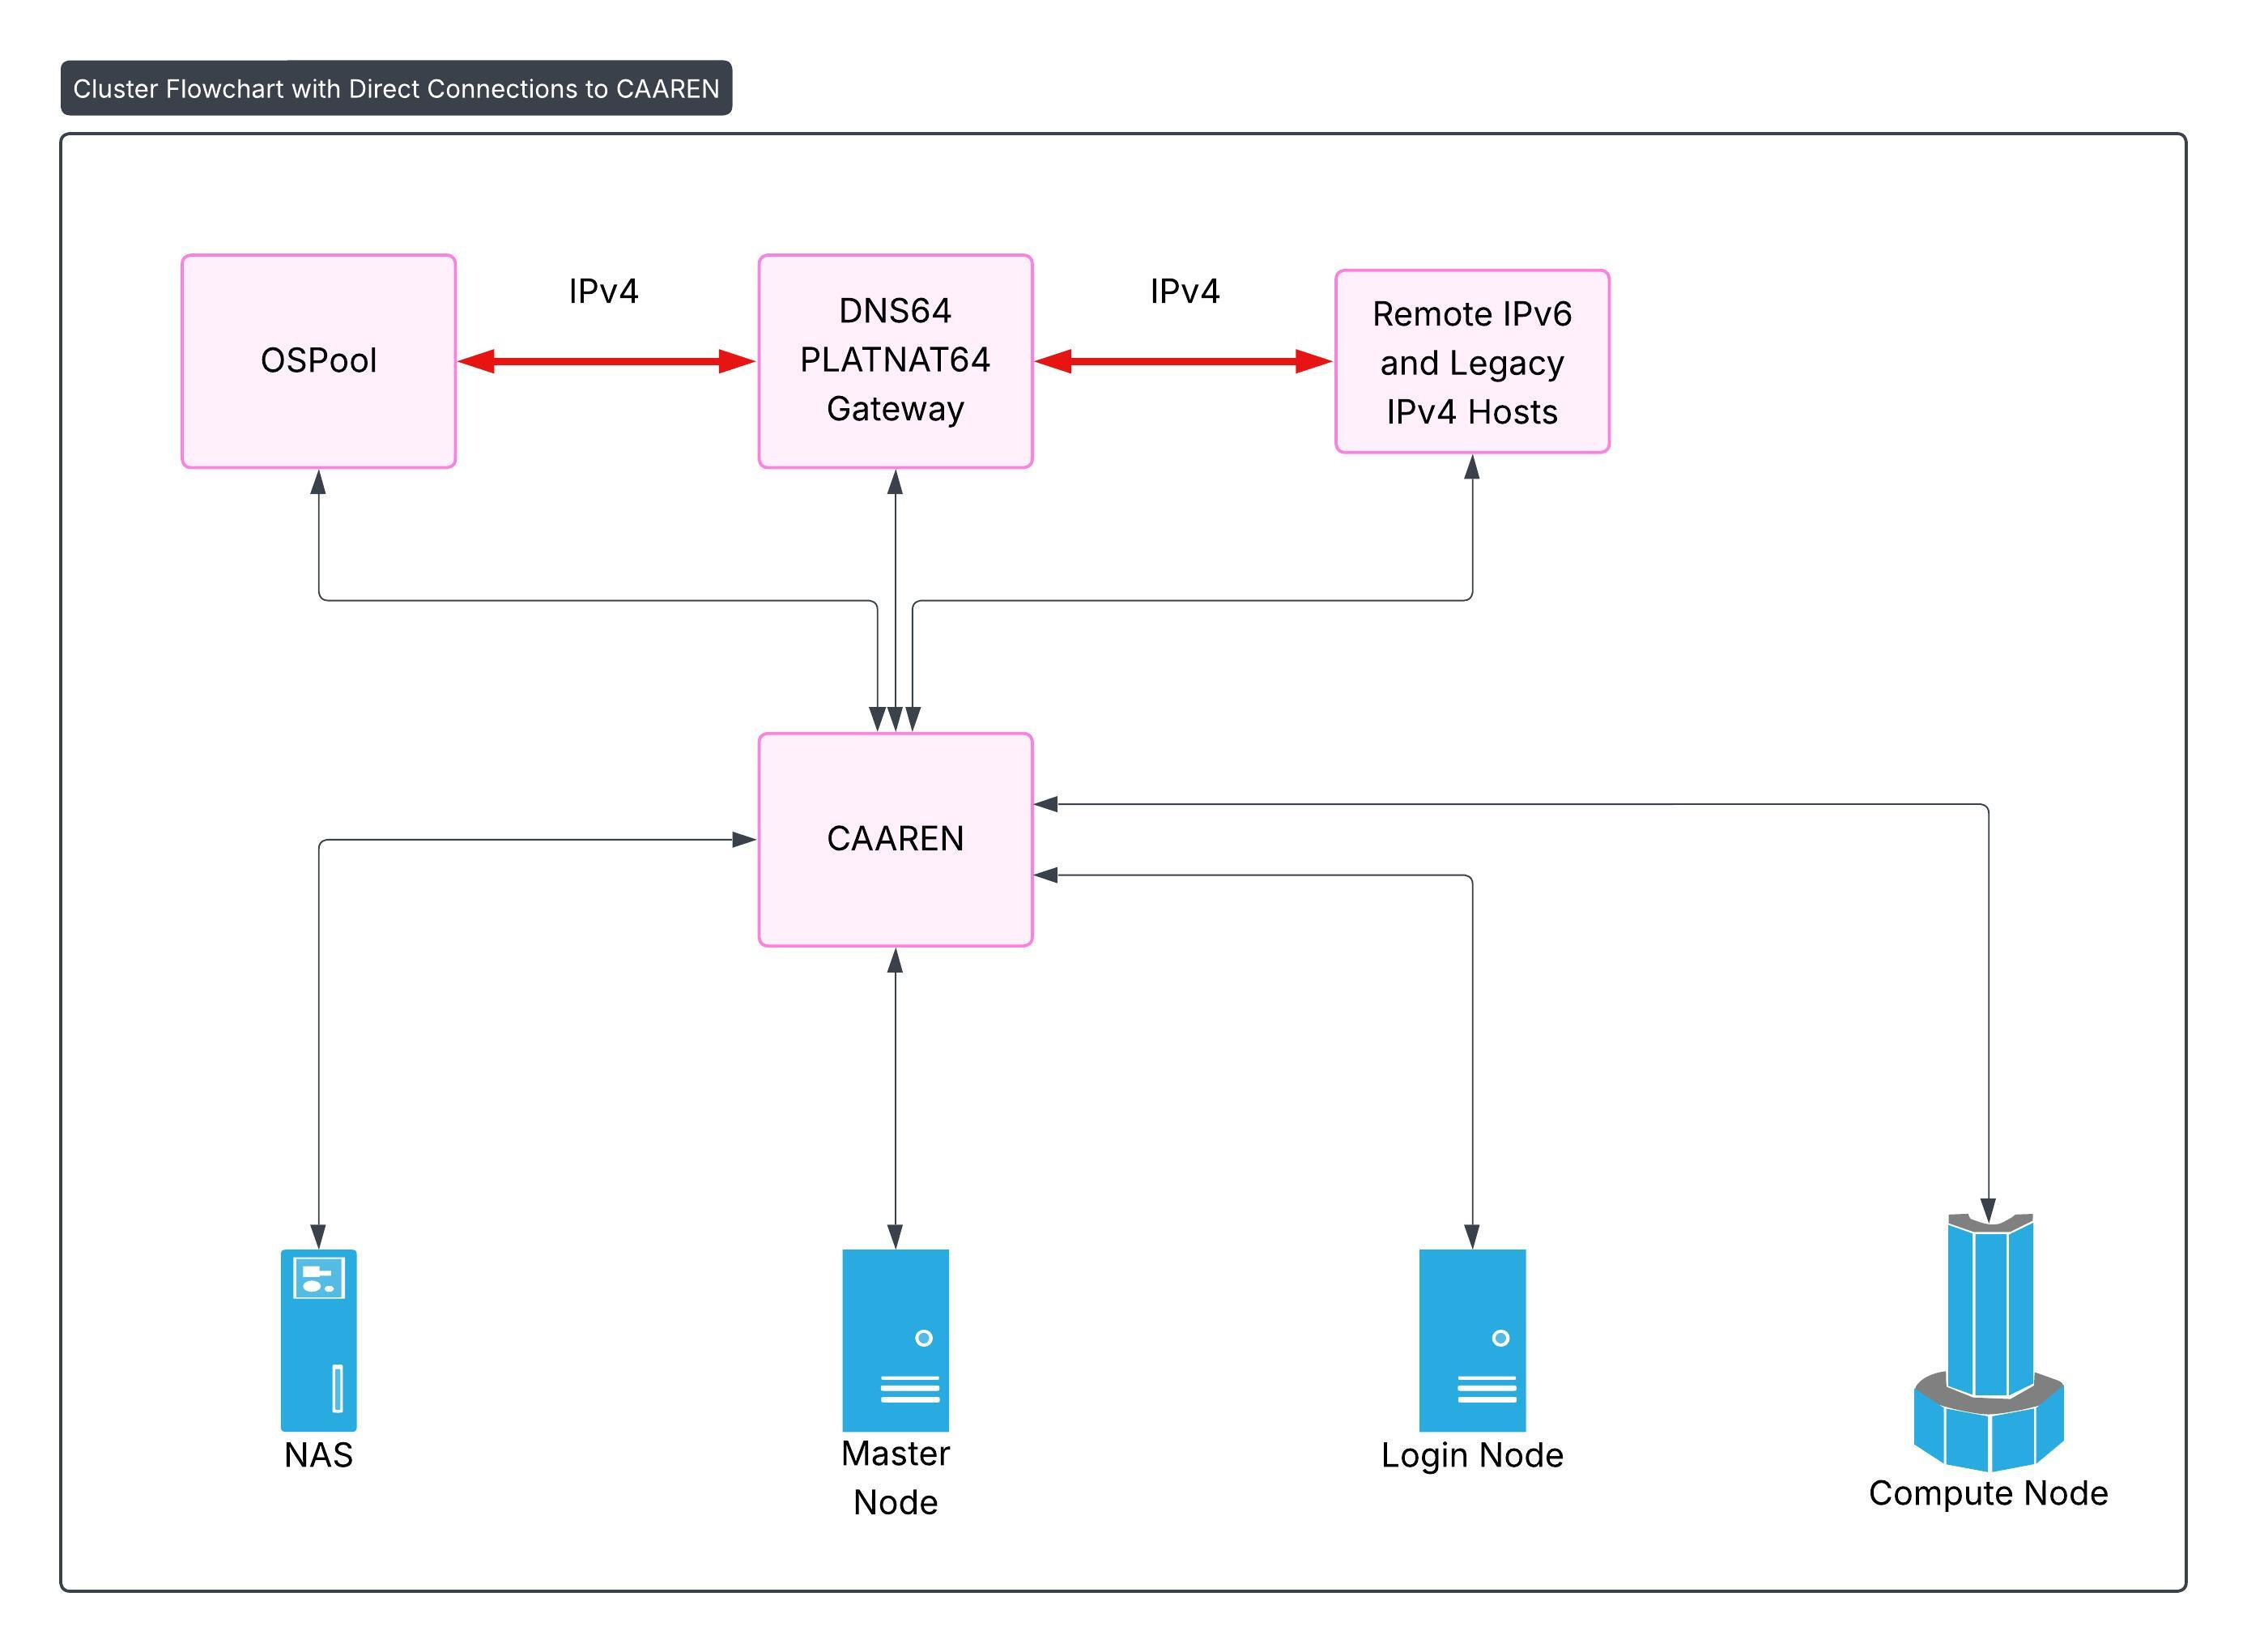
\includegraphics[width=0.49\linewidth]{Viper_Network.jpeg}
  \caption{Essential network architecture of the Viper IPv6-only implementation.}
  \label{fig:viper-network}
\end{figure}


\section{HTCondor Configuration and IPv6 Deployment}

All HTCondor components are configured to operate over IPv6 only. The following key values were set on each node via overlay.

\subsection*{Access Point and Central-Manager IPs}
Note that the addresses below are reserved for documentation and used for illustrative purposes; they will need to be updated for site-specific networks.  
\begin{center}
\small
\begin{tabular}{|l|l|}
\hline
\textbf{Role} & \textbf{IPv6 Address} \\
\hline
Central-Manager (CONDOR\_HOST) & \texttt{2001:db8:0:1::200} \\
Submit/Access Point & \texttt{2001:db8:0:1::100} \\
\hline
\end{tabular}
\end{center}

\subsection*{/etc/condor/config.d/10\_ipv6.conf}
\begin{lstlisting}
# submit/access point
UID_DOMAIN = 2001:db8:0:1::100

# central-manager
CONDOR_HOST = 2001:db8:0:1::200

NETWORK_INTERFACE = eno1
ENABLE_IPV6 = true
PREFER_IPV6 = true
ENABLE_IPV4 = false

ALLOW_READ = 2001:db8:0:1::/64
ALLOW_WRITE = 2001:db8:0:1::/64
ALLOW_NEGOTIATOR = 2001:db8:0:1::/64
ALLOW_ADVERTISE_STARTD = 2001:db8:0:1::/64
\end{lstlisting}

\subsection*{/etc/condor/config.d/20\_role.conf}
\begin{lstlisting}
# central-manager
COLLECTOR_HOST = [2001:db8:0:1::200]:9618
\end{lstlisting}

\section{DNS64, NAT64, and the Role of CLAT}

Viper operates in an IPv6-only environment so some measures are required to enable connectivity to legacy IPv4 hosts and applications. This is achieved through a combination of DNS64, NAT64, and CLAT, an implementation of 464XLAT~\cite{464xlat}.

DNS64 and NAT64 are required for accessing upstream OSG services, Git repositories, and software mirrors that remain IPv4-only.
\subsection*{DNS64 and NAT64}

\begin{itemize}[leftmargin=*,label=--,itemsep=1pt]
  \item \textbf{DNS64:} When an IPv6-only host makes a DNS request for an A record (IPv4), a DNS64-enabled resolver synthesizes an AAAA record using a configured NAT64 prefix, often \texttt{64:ff9b::/96}, but in the case of Viper an external NAT64 gateway was used.
  \item \textbf{NAT64:} The NAT64 gateway intercepts IPv6 packets destined for these synthesized addresses and translates them to the corresponding IPv4 address, enabling IPv4 interoperability.
\end{itemize}


  
\subsection*{CLAT for Application Compatibility}

Some applications do not support IPv6,  including those that bind to literal,  or hardcoded IPv4 addresses. To address this limitation, Viper utilizes the following:

\begin{itemize}[leftmargin=*,label=--,itemsep=1pt]
  \item \textbf{CLAT (Customer-side Translator):} An open source implementation \cite{clatd} of 464XLAT~\cite{464xlat}, \texttt{CLATD} allows IPv4-only applications to operate in Viper's  IPv6-only environment.  \texttt{CLATD} orchestrates the translation of IPv4 socket calls into IPv6, which are then handled by Viper’s provider-side translator (PLAT)—the NAT64 gateway responsible for bridging to legacy IPv4 services.
  \item \textbf{Implementation:} On Viper, \texttt{CLATD} runs on each node and provides its own instance of \texttt{TAYGA}, an out-of-kernel stateless NAT64 daemon. \texttt{CLATD} (and \texttt{TAYGA}) are integrated at boot through systemd units within overlays. 
\end{itemize}

Note, in a dual-stack environment (e.g., while transitioning from legacy to IPv6) it is important that HTCondor not attempt to bind to the virtual \texttt{clat} interface for intra-daemon communication. It is typically sufficient to specify the appropriate interface by setting \texttt{NETWORK\_INTERFACE} and redirecting all other IPv4-bound traffic to the \texttt{clat} interface.  


Together, DNS64, NAT64, and CLAT allow IPv6-only nodes to maintain operational capability with legacy IP hosts and applications. 

\section{Results}
\begin{itemize}
\item Viper has been integrated successfully into the OSPool. 
\item Despite signaling ENABLE\_IPV4 = false and PREF
\end{itemize}

\section{Conclusions}



\section*{Appendix: Site-Specific Notes}
\subsection{Installing \texttt{CLATD}}
Due to the stateless nature of Viper's execute images, installing \texttt{CLATD} into an image presents an issue. The \texttt{CLATD} installation procedure doesn't handle \texttt{TAYGA} installation correctly if it cannot start or run daemons, as is the case with modifying an image.  For installation on Viper,  the \texttt{CLATD} Makefile was modified and \texttt{TAYGA} installed separately.  Viper's minimal \texttt{CLATD} Makefile is,


\begin{lstlisting}
DESTDIR=
PREFIX=/usr
SYSCONFDIR=/etc

DNF_OR_YUM=/usr/bin/dnf
SYSTEMCTL=/usr/bin/systemctl

all:

install:
	install -D -m0755 clatd $(DESTDIR)$(PREFIX)/sbin/clatd
	pod2man --name clatd --center "clatd - a CLAT implementation for Linux" --section 8 README.pod $(DESTDIR)$(PREFIX)/share/man/man8/clatd.8 && gzip -f9 $(DESTDIR)$(PREFIX)/share/man/man8/clatd.8 || echo "pod2man is required to generate manual page"
	if test -d "$(DESTDIR)$(SYSCONFDIR)/systemd/system"; then install -m0644 scripts/clatd.systemd $(DESTDIR)$(SYSCONFDIR)/systemd/system/clatd.service ; fi
	if test -d $(DESTDIR)$(SYSCONFDIR)/NetworkManager/dispatcher.d; then install -m0755 scripts/clatd.networkmanager $(DESTDIR)$(SYSCONFDIR)/NetworkManager/dispatcher.d/50-clatd; fi

installdeps:
	if test -x "$(DNF_OR_YUM)"; then $(DNF_OR_YUM) -y install perl perl-IPC-Cmd perl-Net-IP perl-Net-DNS perl-File-Temp perl-JSON iproute nftables; fi
\end{lstlisting}

\subsection{HTCondor Configuration}
Issues may arise from using short hostnames derived from \texttt{/etc/hosts} which we avoided by using IPv6 literals for \texttt{CONDOR\_HOST}, \texttt{COLLECTOR\_HOST}, and \texttt{UID\_DOMAIN}.

\begin{thebibliography}{99}
\bibitem{gwu}
The George Washington University. \textit{Research Technology Services – GW IT}. \url{https://it.gwu.edu/research-technology-services}. Accessed June 2025.


\bibitem{caaren}
Capital Area Advanced Research and Education Network (CAAREN). \url{https://caaren.org}. Accessed June 2025.

\bibitem{htcondor}
Thain, D., Tannenbaum, T., and Livny, M. (2005). \textit{Distributed computing in practice: the Condor experience}. Concurrency and Computation: Practice and Experience, 17(2-4), 323–356.

\bibitem{ospool}
Open Science Pool (OSPool). \url{https://osg-htc.org/services/open_science_pool.html}. Accessed June 2025.


\bibitem{warewulf}
Warewulf Project. \textit{Warewulf – Scalable Systems Management for HPC}. \url{https://warewulf.org}. Accessed June 2025.

\bibitem{TCPAO}
Gallo, A., Bonica, R., and Aelmans, M. (2022). \textit{Production Deployment of TCP Authentication Option}. RIPE Labs. \url{https://labs.ripe.net/author/andrew-gallo/production-deployment-of-tcp-authentication-option/}

\bibitem{TreeDN}
Giuliano, L., Lenart, C., and Adam, R. (2025). \textit{TreeDN: Tree-Based Content Delivery Network (CDN) for Live Streaming to Mass Audiences}. RFC 9706. \url{https://tools.ietf.org/html/rfc9706}

%\bibitem{ipv6}
%Deering, S., and Hinden, R. (1998). \textit{Internet Protocol, Version 6 (IPv6) Specification}. RFC 2460. \url{https://tools.ietf.org/html/rfc2460}

%\bibitem{dns64}
%Bagnulo, M., Sullivan, A., Matthews, P., and van Beijnum, I. (2011). \textit{DNS64: DNS Extensions for Network Address Translation from IPv6 Clients to IPv4 Servers}. RFC 6147. \url{https://tools.ietf.org/html/rfc6147}

%\bibitem{nat64}
%Bagnulo, M., Matthews, P., and van Beijnum, I. (2011). \textit{IP/ICMP Translation Algorithm}. RFC 6145. \url{https://tools.ietf.org/html/rfc6145}

\bibitem{464xlat}
Anderson, T., Byrne, C., and Bush, R. (2013). \textit{464XLAT: Combination of Stateful and Stateless Translation}. RFC 6877. \url{https://tools.ietf.org/html/rfc6877}

%\bibitem{juniper-464xlat}
%Juniper Networks. \textit{Connecting IPv4-only Hosts to IPv6 Networks Using 464XLAT}. \url{https://www.juniper.net/documentation/us/en/software/junos/interfaces-adaptive-services/topics/topic-map/ipv4-connect-ipv6-464xlat.html}. Accessed June 2025.

\bibitem{clatd}
Anderson, T. \textit{clatd – A 464XLAT CLAT implementation for Linux}. GitHub repository. \url{https://github.com/toreanderson/clatd}. Accessed June 2025.

\end{thebibliography}

%The following procedures apply specifically to stateless nodes managed using Warewulf overlays. These are not essential for IPv6 deployment in general, but are critical for environments similar to Viper:

%\begin{enumerate}[itemsep=1pt]
%  \item Ensure overlays are chmod’d: \texttt{wwctl overlay chmod condor <filepath> 644}
  %\item Rebuild: \texttt{wwctl overlay build}
%  \item Apply: \texttt{systemctl restart condor} on all nodes
%\end{enumerate}

%Running \texttt{condor\_reconfig} or \texttt{condor\_restart} in the middle of a network transition may yield unpredictable behavior. Full service restarts are recommended.

% Remaining sections to be added: NAT64, DNS64, CLAT, Monitoring challenges, Conclusions, etc.

\end{document}



